\chapter{Szövegfüggvények}
\thispagestyle{empty}

Ebben a kategóriában több tucat függvényt találunk, amelyek
segítségével szövegtartalmú cellákkal végezhetünk
különböző műveleteket.

Az \textbf{ÖSSZEFŰZ} függvény segítségével egyetlen
karakterlánccá egyesíthetjük az  argumentumban megadott
karakterláncokat. Az argumentumok lehetnek cellahivatkozások is.

Az \textbf{AZONOS} összehasonlít két szöveges karakterláncot.
Amikor azok megegyeznek, IGAZ értéket ad vissza. Ez a függvény
különbséget tesz kis- és nagybetűk között.

A \textbf{SZÖVEG.KERES} függvény egy szövegrész karakterláncon
belüli helyzetét adja eredményül. A keresés
kezdőpontját paraméterként adhatjuk meg.  A keresés nem
különbözteti meg a kis- és nagybetűket. A
SZÖVEG.KERES("m";"Mamut")
eredménye 1 lesz, mert a Mamut szó első karaktere  m.

A \textbf{SZÖVEG.TALÁL} függvény szöveget keres egy másikban, és
megadja, hogy hányadik karaktertől kezdődik. Opcionális
paraméterként megadható, hogy a keresés melyik karaktertől
kezdődjön. A keresés megkülönbözteti a kis- és
nagybetűket. A
SZÖVEG.TALÁL("m";"Mamut")
eredménye 3 lesz, mert a kis m betű harmadik a Mamut szóban.

A \textbf{BAL} függvény egy szöveg első karaktereit adja
eredményül. A BAL("rendszer";4) eredménye a ,,rend'' szó lesz. A második
paramétert el is hagyhatjuk, ilyenkor csak az első karaktert adja
eredményül.

A \textbf{JOBB} függvénnyel egy szöveg utolsó karaktereit
jeleníthetjük meg. A JOBB("alma";2) eredménye a ,,ma'' szó lesz.

A \textbf{KÖZÉP} függvény egy karakterlánc egy darabját adja
vissza. A kezdőpozíciót, illetve a karakterek számát a
paraméterek határozzák meg. A KÖZÉP("karaktereit";4;3)
eredménye az ,,akt'' szó lesz.

A \textbf{HOSSZ} függvény egy szövegnek a szóközökkel együtt
vett hosszát adja eredményül.

A \textbf{KISBETŰ} függvény argumentumában megadott szöveg minden
nagybetűjét kisbetűre cseréli.

A \textbf{TNÉV} függvény nagybetűsre változtatja egy
szöveg minden szavának első betűjét.

A \textbf{NAGYBETŰS} függvény argumentumában megadott szöveg minden
kisbetűjét nagybetűre cseréli.

A \textbf{HELYETTE} függvénnyel megadott karaktereket, másikra
cserélhetünk. Szintaxisa: HELYETTE(szöveg; keresendő
szöveg; új szöveg; előfordulás).

A HELYETTE("Varga Pál";"Pál";"Péter")
eredménye Varga Péter lesz, mert a függvény az első
argumentumban megadott szövegben lecseréli a
,,Pál'' minden előfordulását ,,Péter''-re.

A \textbf{CSERE} függvény kicseréli egy karakterlánc
részét egy másik karakterláncra. Szintaxisa: CSERE(szöveg;
pozíció; hossz; új szöveg) A
CSERE("Számológép";5;2;"ít")
eredménye Számítógép. Az 5. pozíciótól két karaktert
lecseréli az ,,ít'' karakterekre.

A \textbf{SZÖVEG} függvény egy számot szöveggé alakít,
megadott formátum szerint. Szintaxisa:\\
SZÖVEG(szám; formátum). A SZÖVEG(39676;"yyyy.mmmm dd.")
függvény a cellában  a következő szöveget eredményezi: 2008.augusztus 16. 

A \textbf{TRIM} függvény eltávolítja a szóközöket egy
karakterláncból, a szavak között csak egy szóköz marad.

A \textbf{RÓMAI} függvény konvertálja a számot római
számmá. Az értéktartománynak 0-3999 között kell lennie.
Szintaxisa: RÓMAI(szám; mód). A mód 0-4 közötti egész
szám, ami az egyszerűsítés  mértékét jelöli. Minél
nagyobb az érték, annál nagyobb a római szám
egyszerűsítése. A RÓMAI(1998;2) eredménye MXMVIII lesz.

Az \textbf{ARABIC}\footnote{Az Excelben nem létezik.} függvény egy római szám értékét adja
meg arab számként. Az értéktartománynak 0-3999 között
szükséges lennie. Az ARABIC(MCLXV) eredménye
1165.

Az \textbf{ÉRTÉK} függvény egy szöveget számmá alakít.
Általában akkor van szükség a használatára, amikor egy
szövegformátumú cella, számot tartalmazó értékével kell
műveletet végrehajtani.  

A \textbf{\&} operátorral összefűzhetünk szövegeket egy
cellában. A
BAL("kézikönyv";4)\&{"labda"}
eredménye a ,,kézilabda''
szó lesz. 


\section{18. feladat}
{\itshape
A munkafüzet A oszlopában nevek vannak. Függvények
segítségével oldjuk meg, hogy a B oszlopban a nevek az esetleges
,,dr. '' vagy ,,Dr. '' előtag nélkül
jelenjenek meg. A nevek közé beírt fölösleges
szóközöket is távolítsuk el.}

Kézenfekvő megoldásnak a HELYETTE függvény használata
tűnne, amivel üres karakterre cserélnénk a megadottakat. Ez a
függvény viszont különbséget tesz kis- és nagybetűk
között.

Vizsgáljunk meg egy másik megoldást. Ellenőrizzük le az A1
cella tartalmának első három karakterét. Amennyiben ez
egyenlő a ,,dr.'' karakterekkel, a
cellában csak a jobbról vett karakterek jelenjenek meg, melyek
száma az eredeti karakterek számától hárommal kevesebb. Ezt
kiszámíthatjuk a \textsf{\textbf{HOSSZ(A1)-3}} kifejéssel. A
,,dr.'' nélküli cellatartalmat a
\textsf{\textbf{JOBB(A1;HOSSZ(A1)-3)}} kifejezés adja meg. A B1
tartalma tehát:
\textsf{\textbf{=HA(BAL(A1;3)=''dr. '';JOBB(A1;HOSSZ(A1)-3);A1)}}
(\ref{18-feladat} ábra).

\begin{figure}[!h]
\begin{center}
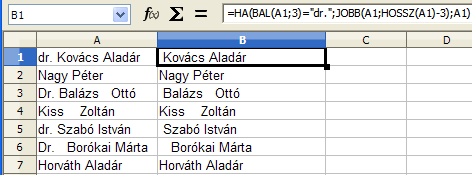
\includegraphics[width=11.354cm]{oocalcv2-img90.png}
\caption{18. feladat}\label{18-feladat}
\end{center}
\end{figure}

Figyeljük meg a kifejezés struktúráját a
Függvénytündér ablakában (\ref{18-feladatIF} ábra). Több beágyazott
függvény használatakor a kifejezés működését segít
megérteni, ha kiválasztjuk valamelyik beágyazott függvényt,
és megvizsgáljuk argumentumait és eredményét.

\begin{figure}[!h]
\begin{center}
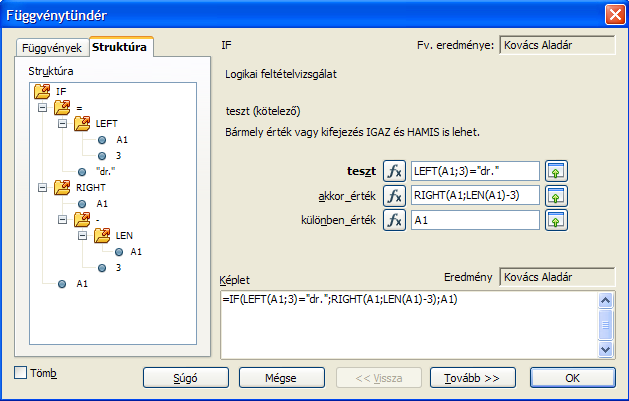
\includegraphics[width=15.999cm]{oocalcv2-img91.png}
\caption{18. feladat --  Függvénytündér -- HA kifejezés struktúra}\label{18-feladatIF}
\end{center}
\end{figure}

A nevekből távolítsuk el a fölösleges szóköz
karaktereket. Az eddigi kifejezés legyen a TRIM függvény
argumentuma. A feladat megoldása \aref{18-feladatMegoldás} ábrán látható.

\begin{figure}[!h]
\begin{center}
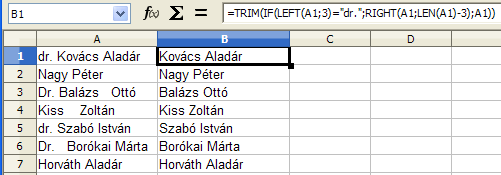
\includegraphics[width=12.254cm]{oocalcv2-img92.png}
\caption{18. feladat -- Megoldás}\label{18-feladatMegoldás}
\end{center}
\end{figure}

Jól látható, hogy mind a vezeték-, mind a keresztnév elé
beírt szóközökből csak egy maradt a B oszlopban.

A \textbf{\&} operátor, amivel szövegeket kapcsolhatunk össze,
segítségünkre lehet számítási feladatok esetén is.
Vizsgáljuk meg ezt a következő feladatban.


\clearpage
\section{19. feladat}

{\itshape
Határozzuk meg, hogy a 12. feladatban vizsgált osztály tanulói
közül hányan értek el az osztályátlag fölötti átlagot.}

A feladat megoldására a DARABTELI függvényt nem tudjuk alapesetben
használni, hiszen a függvény második feltétel argumentuma nem
lehet sem függvény, sem hivatkozás. Még visszatérünk ehhez
a függvényhez, de először oldjuk meg a feladatot logikai
függvények és segédoszlop felhasználásával. Másoljuk a
12. feladat A1:I10 tartományát egy üres munkalapra. A J2
cellába pedig írjuk a következő kifejezést:
\textsf{\textbf{=HA(I2>ÁTLAG(D\$2:H\$10);1;0)}}.
Ez a cella 1-et fog felvenni, ha az első tanuló átlaga az
osztályátlagnál jobb, és 0-át, ha rosszabb. A képletet
másolva számoszlopot kapunk, aminek összege megadja a keresett
eredményt (\ref{19-feladat} ábra).

\begin{figure}[!h]
\begin{center}
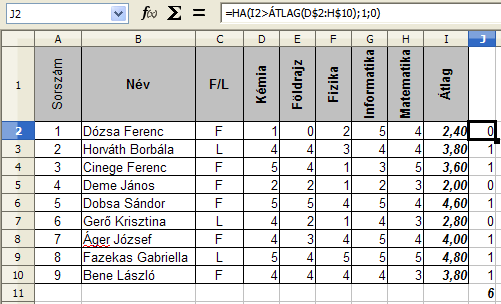
\includegraphics[width=13.254cm]{oocalcv2-img93.png}
\caption{19. feladat}\label{19-feladat}
\end{center}
\end{figure}

A DARABTELI függvény második argumentumában a \textbf{\&}
operátort felhasználva a következő kifejezéssel adhatjuk
meg a feltétel argumentumot:
\textsf{\textbf{">"\&ÁTLAG(D2:H10))}}.
A végleges képlet tehát:
\textsf{\textbf{=DARABTELI(I2:I10;">"\&ÁTLAG(D2:H10))}}.
Írjuk be a képletet a J12 cellába és ellenőrizzük, hogy
ugyanazt az eredményt adja mint az előző esetben.

Az ebben a fejezetben áttekintett függvényeket
\aref{9-fejezetFüggvények} táblázatban találjuk meg.

\begin{table}[!h]
\begin{center}
\caption{A fejezetben tárgyalt függvények}\label{9-fejezetFüggvények}
\begin{tabular}{|m{3cm}|m{8cm}|m{3cm}|}
\hline
\multicolumn{1}{|c|}{\textbf{A függvény}}&
\multicolumn{1}{c|}{\textbf{Funkciója}}&
\multicolumn{1}{c|}{\textbf{A függvény}} \\
\multicolumn{1}{|c|}{\textbf{neve}} & &
\multicolumn{1}{c|}{\textbf{angol neve}} \\
\hline
ÖSSZEFŰZ & Karakterláncokat egyesít. & CONCATENATE\\ \hline
AZONOS & Összehasonlít két szöveges karakterláncot. & EXACT\\ \hline
SZÖVEG.KERES & Egy szövegrész karakterláncon belüli helyzetét adja eredményül.
Kis és nagybetűk között nem tesz különbséget. & SEARCH\\ \hline
SZÖVEG.TALÁL & Egy szövegrész karakterláncon belüli helyzetét adja
eredményül. Kis és nagybetűk között különbséget tesz. & FIND\\ \hline
BAL & Megadja egy szöveg első karaktereit. & LEFT\\ \hline
JOBB & Megadja egy szöveg utolsó karaktereit. & RIGHT\\ \hline
KÖZÉP & Megadja egy karakterlánc egy darabját. & MID\\ \hline
HOSSZ & Szöveg karaktereinek számát adja. & LEN\\ \hline
KISBETŰ & Kisbetűsre alakítja a szöveget. & LOWER\\ \hline
TNÉV & Nagybetűsre változtatja minden szó első betűjét. & PROPER\\ \hline
NAGYBETŰS & Nagybetűsre alakítja a szöveget. & UPPER\\ \hline
HELYETTE & Megadott karaktereket cserél szövegben. & SUBSTITUTE\\ \hline
CSERE & Karaktereket cserél szövegben pozíció alapján. & REPLACE\\ \hline
SZÖVEG & Megadott formátum alapján számot szöveggé alakít. & TEXT\\ \hline
TRIM & Eltávolítja a szükségtelen szóközöket. & TRIM\\ \hline
RÓMAI & Római számra alakít. &  ROMAN\\ \hline
ARABIC & Római számot arab számmá alakít. & ARABIC\\ \hline
ÉRTÉK & Szöveget számmá alakít. & VALUE\\ \hline
\end{tabular}
\end{center}
\end{table}

